\documentclass[11pt,a4paper]{article}
\usepackage[T1]{fontenc}
\usepackage[utf8]{inputenc}
\usepackage{lmodern}
\usepackage{amsmath,amssymb,amsthm,mathtools,mathrsfs}
\usepackage{graphicx,float,xcolor,multicol}
\usepackage[shortlabels]{enumitem}
\usepackage[margin=27mm]{geometry}
\usepackage{microtype,needspace,placeins}
\usepackage{tikz,tikz-cd}
\usetikzlibrary{arrows.meta,calc,positioning,patterns,decorations.pathreplacing}
\usepackage[colorlinks=true,linkcolor=teal,urlcolor=teal,citecolor=teal]{hyperref}
\setlength{\parindent}{0pt}
\setlength{\parskip}{.6em}
\setcounter{secnumdepth}{0}
\allowdisplaybreaks
\raggedbottom
\providecommand{\cross}{\times}
\DeclareUnicodeCharacter{2020}{\ensuremath{\dagger}}
\DeclareMathOperator{\supp}{supp}
\DeclareMathOperator*{\esssup}{ess\,sup}
\providecommand{\chapter}{\section}
\newenvironment{tool}[2]{\subsection*{Tool #1 --- #2}}{}
\newcommand{\ToolRef}[1]{Tool #1}
\newcommand{\FigureTag}[2]{\textit{Figure #1}}
\newcommand{\Result}[1]{\subsection*{#1}}
\newcommand{\Application}[1]{\subsubsection*{Application\if\relax\detokenize{#1}\relax\else\space--- #1\fi}}
\newcommand{\ProofHeading}{\par\textit{Proof.}\space}
\newcommand{\ProofOf}[1]{\par\textit{Proof of #1.}\space}
\newcommand{\RemarkHeading}{\par\textbf{Remark.}\space}
\newcommand{\NoteHeading}{\par\textbf{Note.}\space}
\newcommand{\ExerciseHeading}{\par\textbf{Exercise.}\space}

\graphicspath{{figures/surgeries/}}
\begin{document}
\section*{Classification of Non-Wandering Fatou Components}
% BLOG-CONTENT-BEGIN

    
        Let $f$ be a rational map on the Riemann sphere $\hat{\mathbb{C}}$ with $\deg(f)\geq2$. This post reviews the background needed to classify the periodic Fatou components of $f$ up to conformal equivalence.

\subsection{Background and motivation}
    
        
        Our story begins with two very basic questions - How to study the deformation of a Riemann surface with tools like holomorphic maps at our disposal? What are the consequences of such a study? We shall linger more on the first question, with consequences appearing as instances of the proposed means of study. Let's begin by introducing the objects in the question (historically).

        In the early $20$th century Henri Poincaré and Paul Koebe proved the uniformization theorem. It characterizes Riemann surfaces as quotients of three model surfaces: the unit disc, the complex plane, and the Riemann sphere. More precisely, it says the following:
        
      
        \subsection*{Theorem — Uniformization Theorem, $1907$} Let $S$ be a Riemann surface, then $S$ is conformally isomorphic to a quotient of the form $\hat{S}/\Gamma$, where $\hat{S}$ is necessarily conformally isomorphic to either the unit disk $\mathbb{D}$, the complex plane $\mathbb{C}$, or the Riemann sphere $\hat{\mathbb{C}}$, where $\Gamma \cong \pi_1(S)$ is a group of conformal automorphisms of $S$ which acts freely and properly discontinuously on the universal cover $\hat{S}$.
        
        
        Later in that era a French mathematician named Paul Montel proved theorems about the normality of a given family of holomorphic functions between hyperbolic surfaces. These results were taken up by the French mathematicians Pierre Fatou and Gaston Julia who saw that normality of the family of forward iterates of self maps $f$, namely the family $\{f^{\circ n}\}_n$, was the right tool to study stability and chaos of the deformation of the domain of $f$ (aka dynamics of $f$). Montel's Theorem along with the Uniformization Theorem reduced the number of Riemann surfaces to consider in the study of deformation: up to equivalence, they are - the Riemann sphere, the complex plane, the punctured plane, the torus, and the rest we shall refer to as hyperbolic surfaces. The dynamics on the hyperbolic surfaces have been completely classified, and handling the torus is elementary. This leaves three principal settings to consider. Among them, polynomial dynamics on the complex plane and the dynamics of holomorphic self maps on the Riemann sphere (i.e. rational maps) have historically seen a lot of interesting progress. Hence, we shall focus on these two\footnote{ Handling functions that have essential singularity at $\infty$ on the complex plane or the punctured plane is extremely difficult.}.     

        If we consider the case of rational maps $f: \hat{\mathbb{C}} \rightarrow \hat{\mathbb{C}}$ with deg$(f) \geq 2$; we can prove that the set $J(f)$ (on which the family $\{f^{\circ n}\}_n$ is not locally normal) is a non-empty, nowhere dense, totally invariant, self-similar, perfect subset of $\hat{\mathbb{C}}$. Therefore, $J(f)$ breaks the set $F(f)$ (on which the family of forward iterates of $f$ is locally normal) into connected components, called the Fatou components, where each component shall turn out to be a hyperbolic surface in its own right. The sets $F(f)$ and $J(f)$ are called the Fatou set and the Julia set of $f$ (respectively). Understanding the dynamics of $f$ shall amount to understanding the Fatou set and the Julia set.


        \begin{figure}[!htb]
            \minipage{0.32\textwidth}
                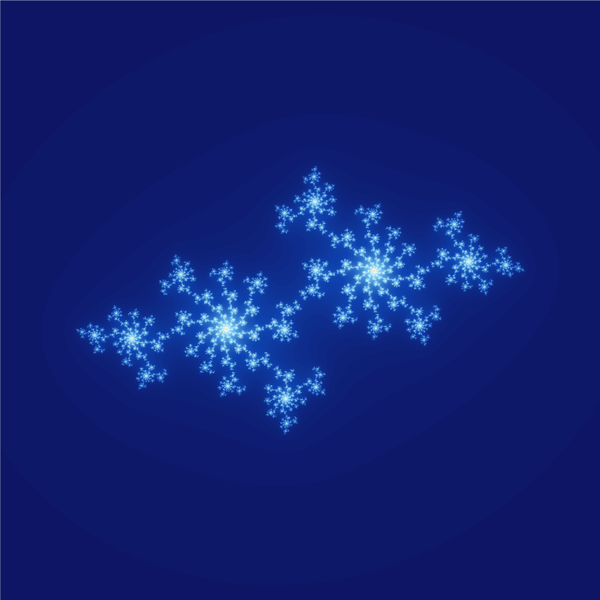
\includegraphics[width=\linewidth]{J1.png}
                
            \endminipage
            \minipage{0.32\textwidth}
                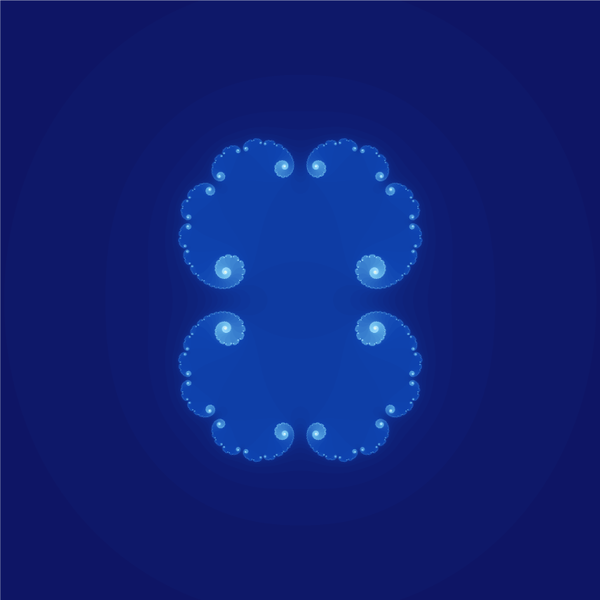
\includegraphics[width=\linewidth]{J2.png}
                
            \endminipage
            \minipage{0.32\textwidth}%
                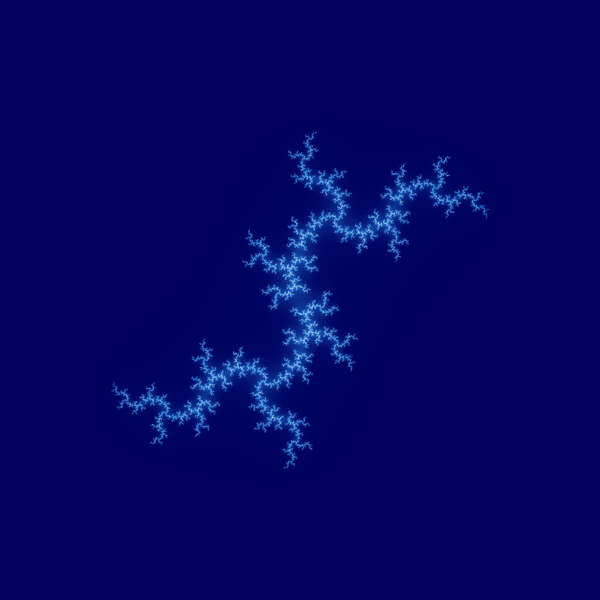
\includegraphics[width=\linewidth]{J3.png}
                
            \endminipage
        \end{figure}


        Below, we shall review the background from complex dynamics with which one will be able to deduce that the Fatou components whose orbits eventually recur can be completely classified (up to conformal equivalence) using the classification theorem of self maps on hyperbolic surfaces. The arguments that go in proving the aforementioned classification theorem cannot capture any information about the Fatou components that keep wandering across the Riemann sphere (if any). This, in spirit, sums up the work of Fatou and Julia.  

        Although their work greatly clarified the stability of rational dynamics, many problems remained open for decades because the necessary tools were unavailable. One of them being the following: 
    
        \subsection*{Conjecture — No Wandering Domain} The orbits of all Fatou components of rational maps of degree at least $2$ are eventually periodic.


        Parallelly, beginning with the work of Herbert Gr\"otzsch, and later contributions from mathematicians like Lars Ahlfors, Oswald Teichm\"uller, Albert Pfluger, and Charles B. Morrey; the right means to loosen the notion of conformality was formulated. Not only that, a general theory around such a notion was also laid out with deep connections to the function theory of Riemann surfaces. At that stage complex dynamics needed just that!  

        Monumental to any theory is the robustness of its classification theorems. In the case of dynamics, to be able to classify, one must first be able to compare or alter the dynamics of $f$ to grasp the parameters that control such things. One cannot alter the dynamics of $f$ within setup of conformality because of its innate rigidity. Therefore, generalizing holomorphic maps was a natural next step (in retrospect). But historically speaking, the loosened notion of conformality (i.e. quasiconformality) entered complex dynamics quite abruptly. 

        Quasiconformal maps (abbreviated as QC-maps) are conformal (i.e angle preserving) up to a bounded error. Hence, QC-maps are much more flexible than holomorphic maps for they don't have to obey the Identity Theorem. In the $1950$s Ahlfors and Bers proved the celebrated Measurable Riemann Mapping Theorem which is essentially the Riemann Mapping Theorem for QC-maps. This theorem yields a way to associate a QC-map to a given holomorphic map. Following such a ductile association one performs a series of alterations in both the domain of the function and the function itself via a mechanism spelled out explicitly by the Surgery Principles. And finally, the crucial step in all such modes of operations is to land back in the category of holomorphic maps, which is done via Weyl's Lemma. All the aforementioned theoretical means to alter the dynamics of $f$ will be developed in \BlogPost{surgical-tools}{Scalpel, Forceps, and other Surgical Tools}.

        \BlogPost{first-surgery}{Sullivan's No Wandering Theorem} gives the first surgical procedure considered here. Inspired by Poincar\'e's deformations of Fuchsian groups into quasi-Fuchsian groups, Dennis Sullivan used quasiconformal maps to prove the No Wandering Domain Theorem. His technique is called \emph{soft surgery}. The two surgeries that follow use a different method, broadly called \emph{cut-and-paste surgery}. These methods alter the dynamics of $f$ in different ways. Cut-and-paste surgery changes parameters such as multipliers, the number of periodic cycles, and rotation numbers by gluing maps with prescribed behaviour after removing suitable sets from their domains. Soft surgery instead changes coordinates quasiconformally. As the \BlogPost{surgical-tools}{discussion of quasiconformal maps} explains, controlled conformal distortion allows the analytic data of the dynamics to vary while the topological structure is preserved.

        This brings us to the raison d’\^etre of this series. Our goal is to present such techniques in dynamics. The theory of distributions, quasiconformal maps, Riemann surfaces, and holomorphic dynamics, though are foundational for such techniques, and that these techniques in itself can't be formulated into a theory; we shall expose the nuances of these techniques which shall then be shown to have the potential of being the future of dynamics. 

        \BlogPost{second-surgery}{The Multiplier Map} aims to prove the following theorem:
        \subsection*{Theorem — Multiplier Map} Let $\Lambda : \Omega \rightarrow \mathbb{D}$ be the multiplier map, where $\Omega$ is a hyperbolic component of period $p$ of the Mandelbrot set. Then $\Lambda$ is a conformal isomorphism.
        
        
        The objects in the theorem will be introduced below. What the theorem roughly says is that certain components of the Mandelbrot set look like bulbs. If one has the following conjecture:
        \subsection*{Conjecture — Hyperbolicity} The interior of the Mandelbrot set is the union of its hyperbolic components.
        
        
        One can make conclusive statements about the topological shape of the Mandelbrot set, and as shall be shown, also its higher dimensional analogues - the Multibrot sets.


        \begin{figure}[htp]
            \centering
            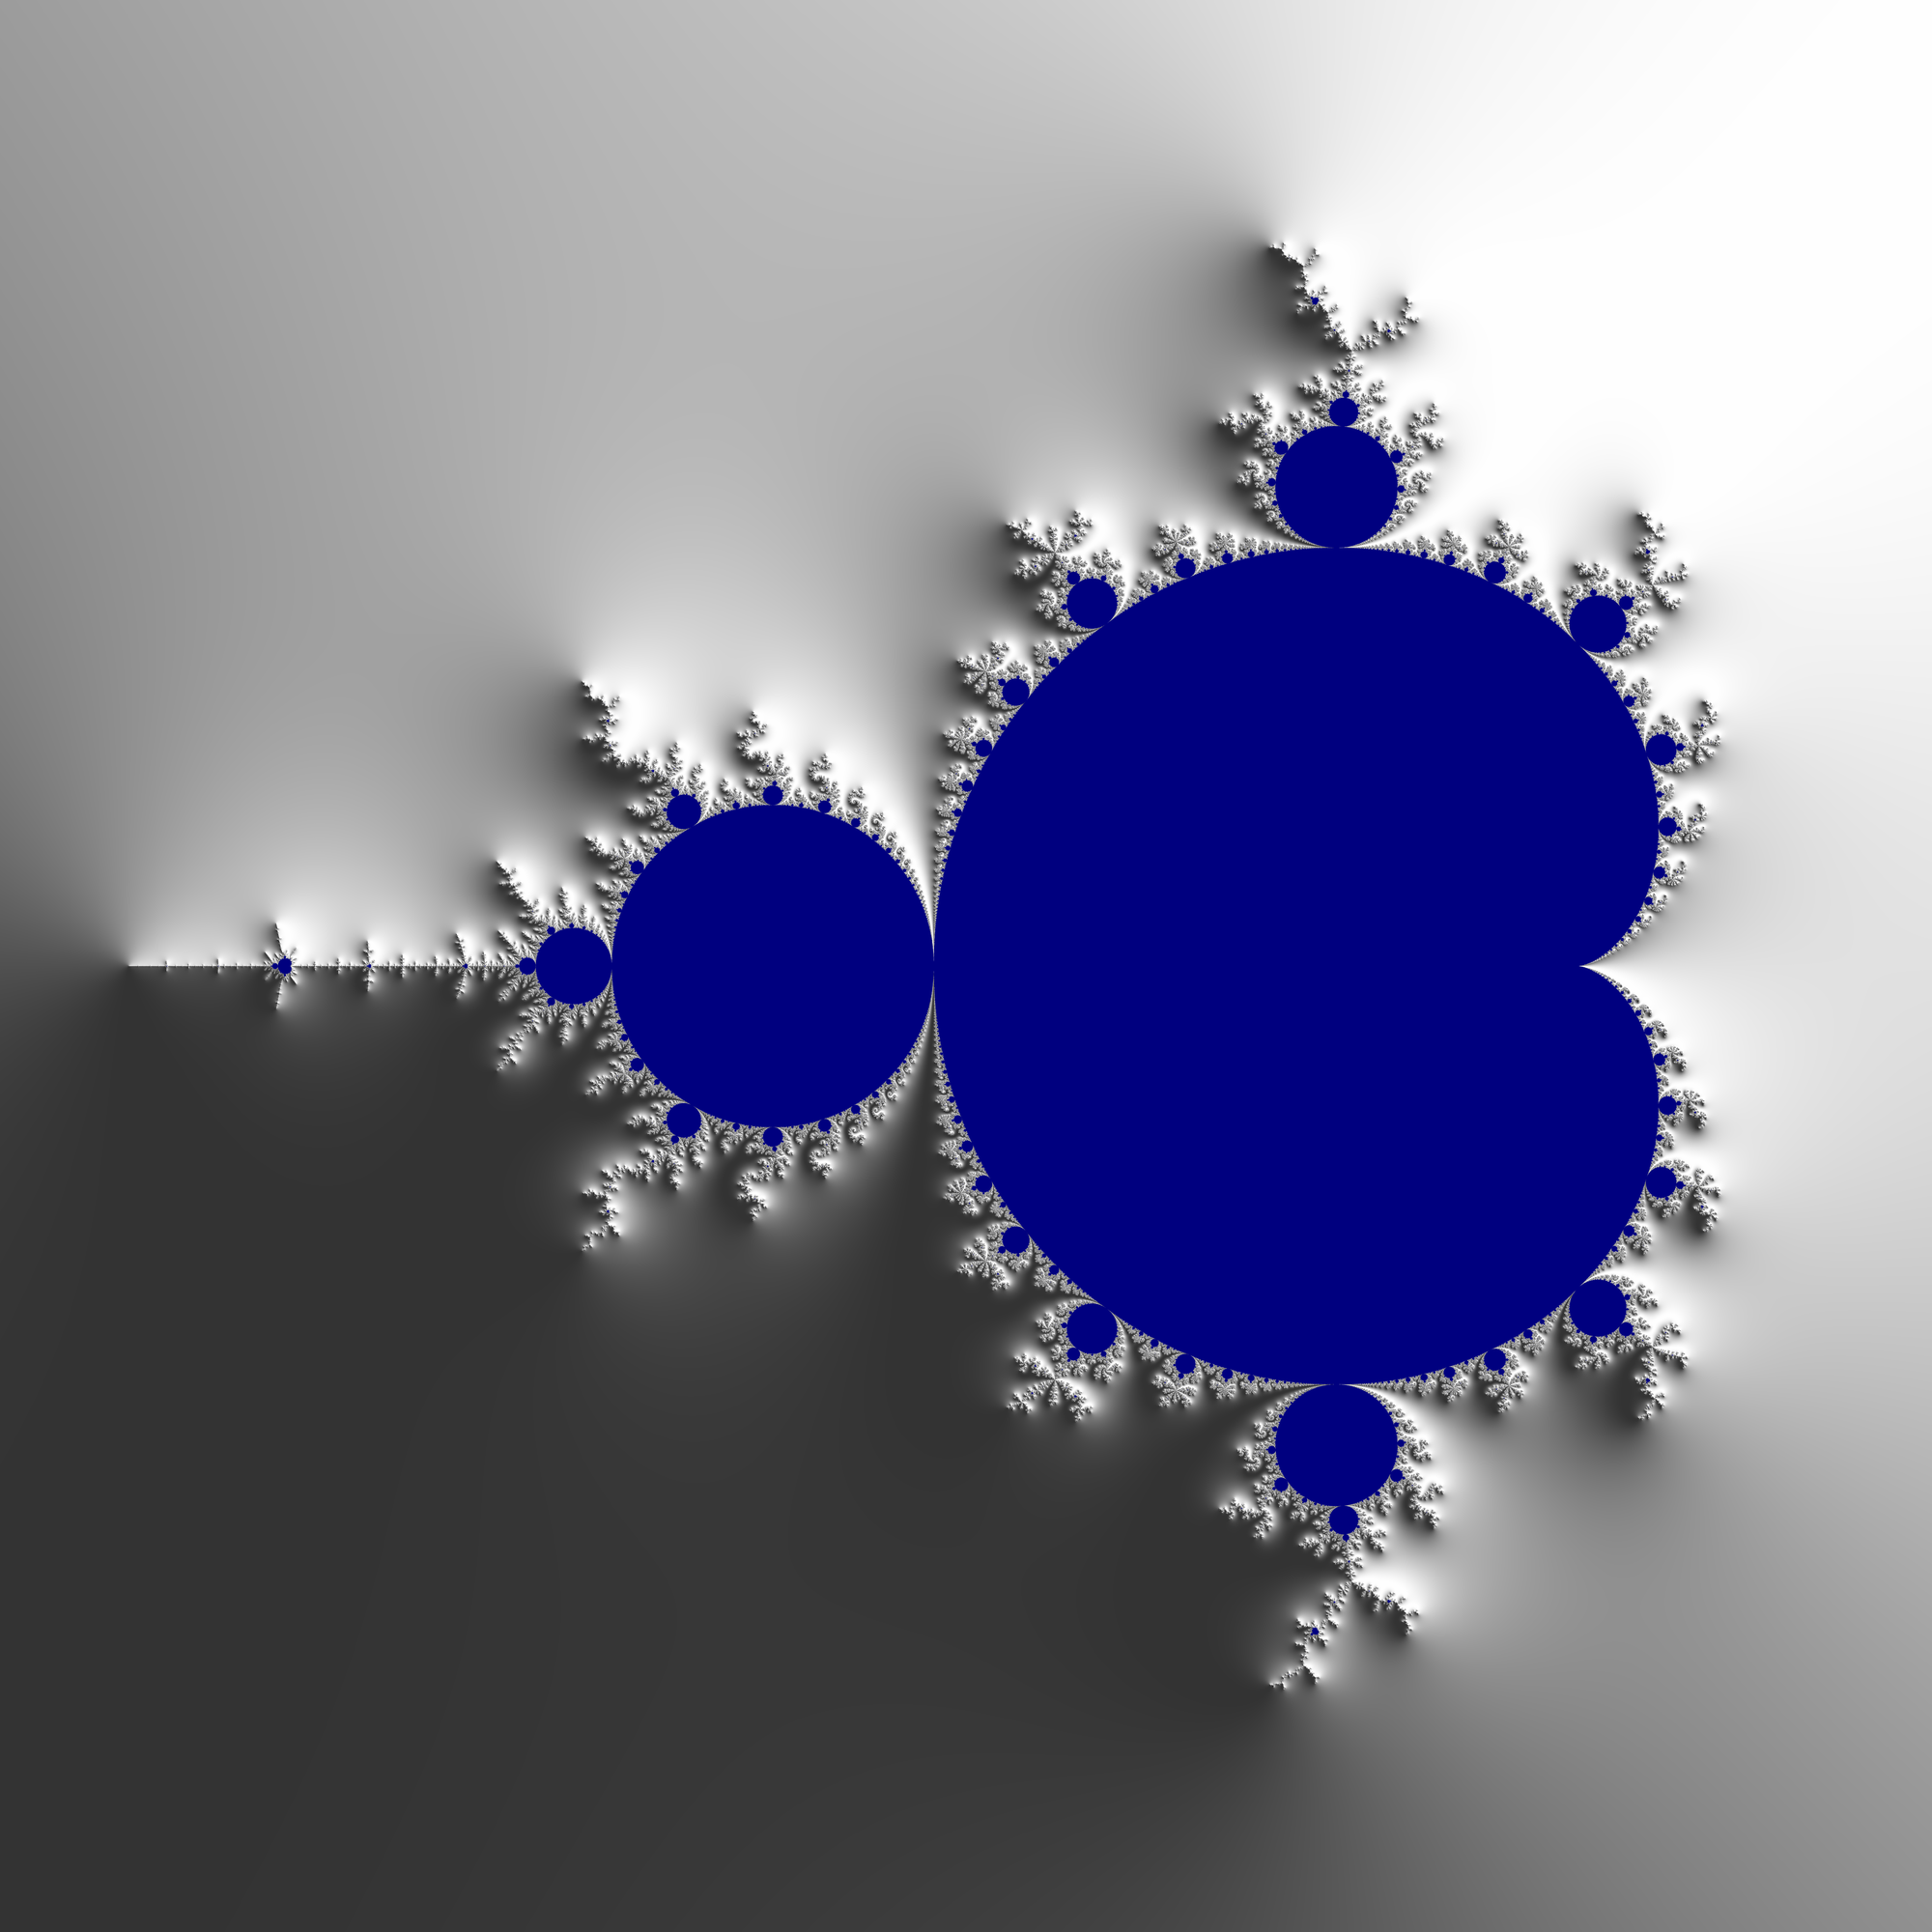
\includegraphics[width=9cm]{M.png}
        \end{figure}


        \begin{figure}[!htb]
            \minipage{0.32\textwidth}
                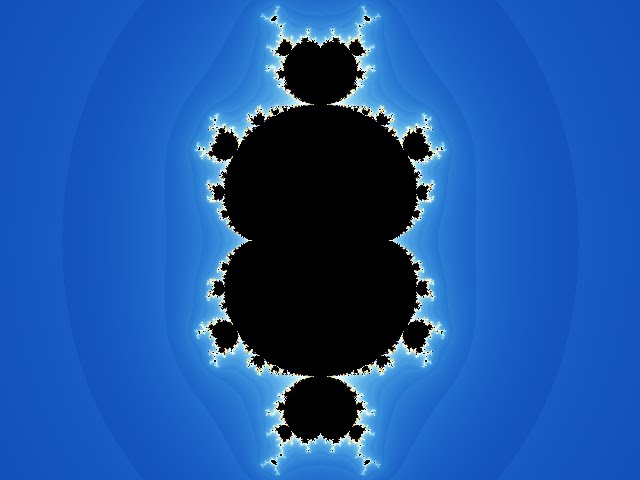
\includegraphics[width=\linewidth]{M1.jpg}
                
            \endminipage
            \minipage{0.32\textwidth}
                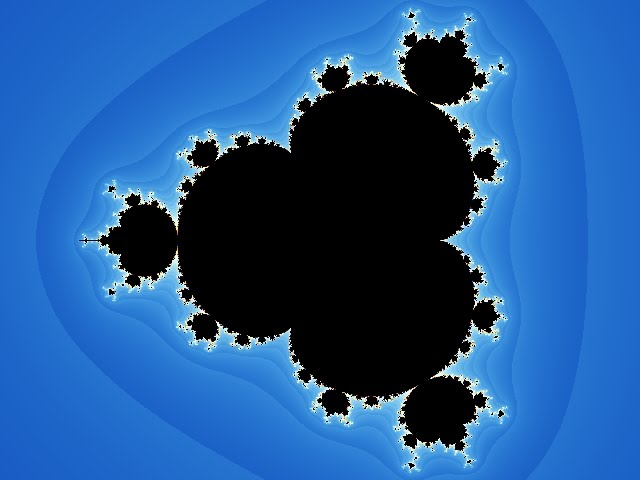
\includegraphics[width=\linewidth]{M2.jpg}
                
            \endminipage
            \minipage{0.32\textwidth}%
                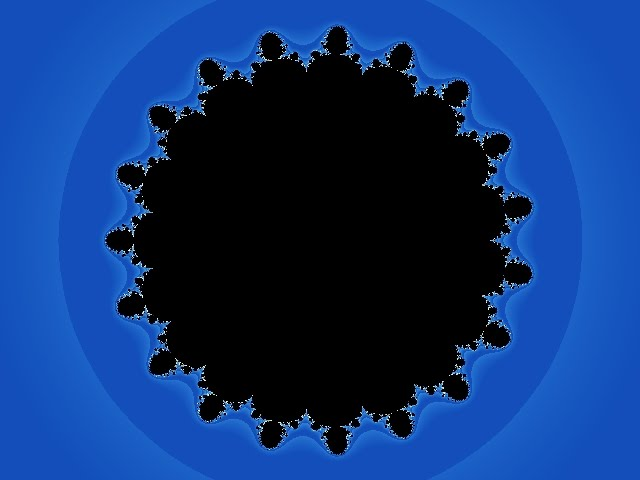
\includegraphics[width=\linewidth]{M3.jpg}
                
            \endminipage
        \end{figure}


        The final post, \BlogPost{third-surgery}{Third Surgery}, discusses the last surgery on our list. There we shall introduce a new object, a group, Mod$(K, f)$, where $K$ is a connected, forward invariant component of $J(f)$. This group in some sense is the group of all quasiconformal homeomorphisms associated to $f$ that commute with $f$ under composition on $K$. Let Aut$(f)$ denote the group of M\"obius transformations that commute with $f$ on $\hat{\mathbb{C}}$. We shall alter the dynamics of $f$ and obtain a new map $g$ (yet again!) to represent the group Mod$(K, f)$ as Aut$(g)$, thereby realizing our objects of interest as subgroups of $PSL_2(\mathbb{C})$. These subgroups also naturally turn out to be finite. Such realizations shall shed light on the periodic components of the Julia set $J(f)$. 

        These three examples, in the absence of a general coherent theory, hammer home the point that Quasiconformal Surgery is still in its infancy. This series deals only with dynamics of very rigid surfaces via maps that are highly regular. Interested readers are invited to pursue this subject in a much more general setting (\cite{katok1997introduction}, \cite{einsiedler2013ergodic}, and \cite{przytycki2010conformal}).

% RESTORED-INTRO-END

\subsection{Dynamical preliminaries}
    
        
        Let us begin with the complex-dynamical background for classifying Fatou components. There are detailed treatments in \cite{milnor2011dynamics}, \cite{mcmullen2016complex}, and \cite{carleson2013complex}. Throughout, $f: S \rightarrow S$ is a holomorphic function and $S$ a Riemann surface (unless otherwise stated).

        By a Riemann surface $S$, we mean a connected complex analytic manifold of complex dimension $1$. In particular, S is a topological manifold of dimension 2 with the transition maps being holomorphic (after appropriately identifying domains in $\mathbb{R}^2$ with domains in $\mathbb{C}$). A function $f: S \rightarrow S'$ between Riemann surfaces $S$ and $S'$ is said to be holomorphic if it is so with respect to the local coordinate maps. If $S = S'$ we shall call $f$ a self map. These self maps induce the concept of change via iteration. For instance, the map $(z \rightarrow z^2) : (1 - \frac{1}{n})\mathbb{D} \rightarrow (1 - \frac{1}{n})\mathbb{D}$ (upon iteration) eventually gobbles up the entire disk of radius $1 - \frac{1}{n}$, whereas the map $(z \rightarrow z^2) : \mathbb{D} \rightarrow \mathbb{D}$ keeps the unit disk as it is. These examples illustrate drastically different dynamics on two Riemann surfaces by the same map, despite one being $\frac{1}{n}$-close to the other for arbitrarily large $n$. 

        Now, given that there are uncountably many Riemann surfaces and that studying dynamics on one gives no approximate information about the dynamics on the other, the problem of classifying Riemann surfaces must be dealt with first. Covering-space theory helps here because Riemann surfaces (by definition) are semi-locally simply connected and locally path-connected and hence admit universal covers. Let $S$ be a Riemann surface with the universal cover $p : \hat{S} \rightarrow S$, then $p$ is a normal cover, hence, $S \cong \hat{S}/G$, where $G$ is a subgroup of Aut$(\hat{S})$ that acts freely and properly discontinuously on $\hat{S}$. With the help of the following theorem \cite{forster2012lectures} one can lift the identification above to the category of Riemann surfaces.
        
        \subsection*{Theorem 2.1}{(Category Lifting)}: Let $S$ be a Riemann surface with $p: \hat{S} \rightarrow S$ a topological covering map. Then there exists a unique complex structure on $\hat{S}$ that turns the map $p$ into a holomorphic covering map. 
        
        
        
        Note that, given a Riemann surface $S$, the moment one has $S \cong \hat{S}/G$, one can forget about $S$ because the identification of the complex structures of $S$ and $\hat{S}$ via quotients is done in a well-defined manner. Therefore, to classify Riemann surfaces one must classify simply-connected Riemann surfaces and the discrete subgroups of their respective automorphism groups\footnote{This object naturally takes up the structure of a Lie group. Hence, studying discrete subgroups of certain Lie groups can yield a great deal of information on such classification theorems.}. By a theorem of Poincar\'e and Koebe \cite{varolin2011riemann} we know that there are only three simply connected Riemann surfaces (up to conformal equivalence), stated explicitly:
        
        \subsection*{Theorem 2.2}{(Uniformization Theorem)}: Any simply connected Riemann surface is conformally isomorphic to one of the following:
        \begin{enumerate}
            \item [(i)]The complex plane $\mathbb{C}$, consisting of complex numbers $z = x+iy$.
            \item [(ii)]The unit disk $\mathbb{D}$, consisting of complex numbers with norm $<1$.
            \item [(iii)]The Riemann sphere $\hat{\mathbb{C}}$, consisting of $\mathbb{C}$ together with $\infty$, wherein $w = 1/z$ is a coordinate map in a neighbourhood around $\infty$. 
        \end{enumerate}
        
        
        
        Riemann surfaces that admit $\mathbb{C},\hat{\mathbb{C}}$, and $\mathbb{D}$ as their universal covers are called Euclidean, Spherical, and Hyperbolic (respectively). If $G < $ Aut$(\hat{\mathbb{C})}$ acts properly discontinuously then by compactness $G = {0}$. Therefore, there is only one Spherical surface, and that is the Riemann sphere. Similarly, one can handle the case of Euclidean surfaces by noting that $G < $ Aut$(\mathbb{C}) (\cong \mathbb{C}^*\times\mathbb{C})$ is abelian and torsion free, and as the action of $G$ on $\mathbb{C}$ is a covering space action, it can't have rank $\geq 3$, for the orbits of points in $\mathbb{C}$ will then be dense. So, $G$ is isomorphic to ${0}$, $\mathbb{Z}$, or $\mathbb{Z}\times\mathbb{Z}$. Finally, up to equivalence, we have the following surfaces to study - the Riemann sphere, the complex plane, torus, cylinder (or the punctured plane), and hyperbolic surfaces. Of these, hyperbolic surfaces offer significantly more mathematical information to dynamics than the others in the lot.

        So, let us handle hyperbolic surfaces first. We propose to do that by answering the following questions:
        \begin{enumerate}
            \item Why care about hyperbolic surfaces?
            \item What are some of its relevant features?
            \item What has all this got to do with complex dynamics?
        \end{enumerate}
        
        
        The answer to the first question is rather simple - \textbf{hyperbolic surfaces are found in abundance}. As can be inferred from the discussion above, all Riemann surfaces with non-abelian fundamental group must be hyperbolic. In fact, there are only 4 Riemann surfaces (up to equivalence) that aren't hyperbolic. In addition, it must also be noted that a sufficiently small domain of a given Riemann surface is hyperbolic. Indeed, fix a Riemann surface $S$, if $S$ is not hyperbolic then $S$ is one of the four model surfaces, deleting three points from any of them would leave a non-abelian fundamental group, hence the resulting surface must certainly be hyperbolic. If $S$ was hyperbolic to begin with and you delete two points from it, it can't be compact, hence it must either be the plane or the punctured plane. It can't be the plane, for $S$ must then be simply-connected, and the fundamental group of a doubly punctured disk isn't abelian. It can't be a punctured plane, for lifting the inclusion map $S\backslash\{p, q\} \hookrightarrow S$ to its respective universal covers would yield a non-trivial holomorphic map from $\mathbb{C}$ to $\mathbb{D}$ contradicting Liouville's Theorem. Therefore, any Riemann surface with three or more punctures is hyperbolic.

        It is a brilliant insight of Riemann that to be able to do geometry on a manifold $M$ one basically needs a symmetric, positive definite, bilinear form on the tangent space $T_pM$ that varies smoothly with $p$. Such inner-products lead to distances, geodesics, angles, curvature, and they can be easily arranged (by locally pushing metrics on $\mathbb{R}^n$ to $M$, and patching it up via partitions of unity). To answer the second question one needs to introduce some such geometry in the setup. Hence, we will be interested in imposing a Riemannian manifold structure on our hyperbolic surface $S$, but not through arbitrary metrics; we will demand this change of category to preserve Aut$(S)$ as Riemann surfaces. Let us first impose such a metric on $\mathbb{H}$, the Poincar\'e upper-half plane, and later filter it for its quotients.
        
        \subsection*{Theorem 2.3}{(Poincar\'e Metric on $\mathbb{H}$)}: There exists a unique (up to multiplication by a constant) Riemannian metric on $\mathbb{H}$ which is invariant under all elements of Aut$(\mathbb{H})$.
        
        
        
        So, all elements $g \in$ Aut$(\mathbb{H})$ under such an invariant metric shall be isometries of $\mathbb{H}$. This is an instance of a general correspondence between Lie groups and symmetric spaces. In that, any left invariant metric on the Lie group turns it into a symmetric space, and the group of isometries of a symmetric space naturally admits a Lie group structure. 

        A symmetric Riemannian metric looks like -  $g_{11}dx\otimes dx + 2g_{12}dx\otimes dy + g_{22}dy\otimes dy$. Now, given a conformal map, $f = u + iv$, which transfers the $(dx, dy)$ tangent plane to $(du, dv)$ tangent plane, we have,
        $$\begin{pmatrix} du\\dv
            \end{pmatrix} = \begin{pmatrix} u_x & u_y\\ v_x & v_y \end{pmatrix} \begin{pmatrix} dx\\dy \end{pmatrix}$$


        Cauchy-Riemann equations yield the following form for the metric altered by $f$ $$du\otimes du + dv\otimes dv = (u_x^2 + v_x^2)dx\otimes dx + (u_y^2 + v_y^2)dy\otimes dy$$
        
        
        Thus the following definition is very natural.
        \subsection*{Definition 2.4}{(Conformal Metric)}: A metric $ds^2$ (which stands for $ds\otimes ds$) $= g_{11}dx^2 + 2g_{12}dxdy + g_{22}dy^2$ will be called conformal iff $g_{11} = g_{22}$ and $g_{12} = 0$.
        
        
        
        The invariant metric on $\mathbb{H}$ whose existence is guaranteed by Theorem 2.3 turns out to be conformal, hence it must be unique up to multiplication by a constant. A conformal metric looks like $ds^2 = \gamma(x+iy)^2(dx^2 + dy^2)$, the norm on tangents given by such a metric will be of the form - $\gamma(x+iy)\sqrt{dx^2 + dy^2} = \gamma(z)|dz|$. Using the Cayley transform $\frac{z+i}{z-i}$, one can transfer the invariant metric on $\mathbb{H}$ to an invariant metric on $\mathbb{D}$, which will then take the form $ds = (\frac{2}{1 -|z|^2})|dz|$. Let us use this to construct a metric on $\mathbb{D}/\Gamma$, where $\Gamma <$ Aut$(\mathbb{D})$ ($\cong PSL_2(\mathbb{R})$) is discrete.

        Let $S$ be a hyperbolic surface and $p: \mathbb{D} \rightarrow S$ be its universal cover. For $y \in S$, let $U_y$ be an evenly covered neighbourhood of $y$ in $S$. Choose $V_a$ open in $\mathbb{D}$ such that $p_{\big|V_a}: V_a \rightarrow U_y$ is a biholomorphism. Set $\gamma_a(p_{\big|V_a}) = \frac{\rho(z)}{|p'(z)|}$, where $\rho(z)|dz|$ is the invariant metric on $\mathbb{D}$. Patch it up via $\{\xi_y\}_y$ (a partition of unity subordinate to the open cover $\{U_y\}_y$) by setting the following metric on $S$:
        $$ds^2 = \sum_{y}{\xi_y(\gamma_a(p_{\big|V_a}(z)))^2(dx^2 +dy^2)}$$
        
        It remains to check that the pushforward metric is well-defined. Let $x,a \in p^{-1}(y)$, since $p$ is a normal covering, $\exists \phi$, $\phi: \mathbb{D} \rightarrow \mathbb{D}$, a deck transformation such that $p = \phi \circ p$ and $\phi(x) = a$. Chain rule and the fact that $\phi$ is a M\"obius transformation gives:
        $$p'(a) = p'(x)\phi'(a),$$
        $$|\phi'(a)| = \frac{1 - |x|^2}{1 - |a|^2} = \frac{\rho(a)}{\rho(x)}$$
        
        Therefore,
        $$\frac{\rho(a)}{|p'(a)|} = \frac{\rho(x)}{|p'(x)|}$$
        
        $\Rightarrow \gamma_a(p_{\big|V_a}(z)) = \gamma_x(p_{\big|V_x}(z))$. This induced Riemannian metric on the hyperbolic surface $S$ shall be referred to as the Poincar\'e metric which shall lead to (as was pointed before) distances, geodesics, angles, and curvature. 
        
        \subsection*{Lemma 2.5}{(Completeness Lemma)}: Let $S$ be a hyperbolic surface and let dist$_S$ denote the Poincar\'e distance on $S$. Then:
        \begin{enumerate}
            \item [(a)] $(S,$ dist$_S)$ is a complete metric space.
            \item [(b)] There exists a geodesic joining any two points of $S$.
        \end{enumerate}
        
        
        
        The key property is that the Poincar\'e distance on a hyperbolic surface is non-increasing under holomorphic maps.
        
        \subsection*{Theorem 2.6}{(Pick's Theorem)}: Let $S$, $S'$ be hyperbolic and $f: S \rightarrow S'$ be holomorphic. Then:
        \begin{enumerate}
            \item $f$ is a conformal isomorphism, in particular an isometry.
            \item $f$ is a covering map, that is, a local isometry.
            \item $\forall$ compacts $K$, $f_{\big|K}$ is a contraction mapping. 
        \end{enumerate}
        
        
        
        Pick's theorem makes the relevance of hyperbolic surfaces to dynamics evident. The Uniformization Theorem classifies simply connected Riemann surfaces; Pick's theorem then controls how holomorphic maps change hyperbolic distance. Iterating this idea leads to the classification of periodic Fatou components. Along the way, we make the notions of order, chaos, and dynamics precise.

        In this subject one is interested in studying how iterates of a self map $f$ deform the surface $S$. This amounts to studying the orbits of individual points under $f$, that is, the sequence - $\{f^{\circ n}(z)\}_n$, for a given $z \in S$. For instance, consider the map $(z \rightarrow z^n): \mathbb{C} \rightarrow \mathbb{C}$, it is visually clear that on the set of points with norm either $(< 1)$ or $(> 1)$, the iterates of the map behave in a stable and predictable manner. Indeed, if one embeds $\mathbb{C} \hookrightarrow \hat{\mathbb{C}}$, then it can easily be seen that the points $0$ and $\infty$ uniformly attract the points in the set mentioned above. But the points on the unit circle with irrational arguments are spun across in an erratic manner. Therefore, to capture both the following should be expected:
        
        \subsection*{Definition 2.7}{(Normal Family)}: A sequence $\{f_i\}_i$ of holomorphic functions from a Riemann surface $S$ to a Riemann surface $T$ will be said to converge locally uniformly if for every point of $S$ one has a neighbourhood $N$ such that the sequence $\{f_i\big|_N\}_i$ converges uniformly (or equivalently, it converges uniformly on compacts). The same sequence will be said to diverge locally uniformly from $T$ if for every compact set $K \subset S$ and $K' \subset T$, $f_n(K)$ and $K'$ are eventually disjoint.
        A collection $\mathcal{F}$ of holomorphic maps between $S$ and $T$ will be called normal if for every infinite sequence of $\mathcal{F}$ we have a subsequence that either converges locally uniformly or diverges locally uniformly. 
        
        
        
        With this definition we have the following two crucial lemmas as consequences of Pick's Theorem.
        
        \subsection*{Lemma 2.8}{(Hyperbolic Compactness)}: If $S$ and $T$ are hyperbolic, then every family $\mathcal{F}$ of holomorphic maps from $S$ to $T$ is normal.
        
        
        \subsection*{Lemma 2.9}{(Ball Convergence)}: Suppose $S\subset S'$ are Riemann surfaces with $S$ hyperbolic, and let $\{p_n\}_n$ converge in $S'$ to a boundary point $\hat p\in\partial S$. For every fixed $r>0$, the hyperbolic balls of radius $r$ centred at $p_n$ converge uniformly to $\hat p$.
        
        
        \begin{figure}[ht!]
        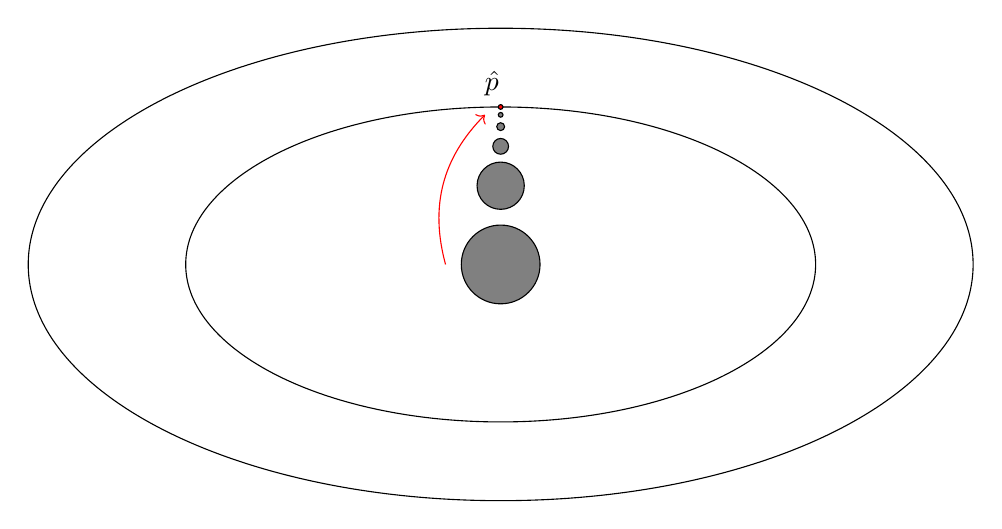
\begin{tikzpicture}
        \draw (0,0) ellipse (6cm and 3cm);
        \draw (0,0) ellipse (4cm and 2cm);
        \draw (0,0) circle (0.5cm)[fill = gray];
        \draw (0,1) circle (0.3cm)[fill = gray];
        \draw (0,1.5) circle (0.1cm)[fill = gray];
        \draw (0,1.75) circle (0.05cm)[fill = gray];
        \draw (0,1.9) circle (0.03cm)[fill = gray];
        \draw (0,2) circle (0.03cm)[fill = red];
        \node[text width=3cm] at (1.3,2.3) {$\hat{p}$};
        \draw [->,red] (-0.7, 0) to [bend left] (-0.2,1.9);
        \end{tikzpicture}
        \end{figure}
        
        
        These two lemmas will be used repeatedly for they say something phenomenal about the dynamics of hyperbolic surfaces. They say that self maps on hyperbolic surfaces show no chaotic behaviour whatsoever, even along the boundary! This knowledge about stability on hyperbolic domains will be used to study stability of deformations in general. Thus, \textbf{hyperbolic surfaces are not only objects of study but also tools in themselves.}

        The stage is now ripe to formally introduce stability, chaos, dynamics, and state the classification theorem for dynamics on hyperbolic surfaces. 
        
        \subsection*{Definition 2.10}{(Stability)}: Given a holomorphic function $f: S\rightarrow S$ on a Riemann surface $S$. Let $F(f)$, the Fatou set of $f$ be the union of all open sets $U \subseteq S$ such that $\{f_{\big|U}^{\circ n}\}_n$ is a normal family. We say that $f$ deforms the set $F(f)$ in a stable manner.
        
        
        \subsection*{Definition 2.11}{(Chaos)}: Given a holomorphic function $f: S\rightarrow S$ on a Riemann surface $S$. Let $J(f) := S\backslash F(f)$ be the Julia set of $f$. Then we say that $f$ deforms the set $J(f)$ chaotically. 
        
        
        
        By dynamics, we mean the structure of the sets $J(f)$ and $F(f)$, be it in the category of sets, topological spaces, Riemann surfaces, or Riemannian manifolds. Having introduced normality as the right means to capture stability let us probe further on what means one should adopt to study dynamics on a given surface.

        There is a general philosophy which speaks of orbits of critical points, fixed points, and periodic points as prime governors of dynamics\footnote{This doesn't all apply for maps in general, at some stage one must restrict oneself to the case of rational maps, or worse, polynomials.}. Here's why that should surprise you: If $f: \mathbb{C} \rightarrow \mathbb{C}$ is holomorphic and say you know the zeroes and poles of $f$. Basic one variable complex analysis will tell you that you can by and large determine the function $f$. To be specific, if $z_0$ were a zero, then if you know $\{f^{(n)}(z_0)\}_n$. You know that,
        $$f(z) = \sum_{n \geq 0}^{\infty}{\frac{f^{(n)}(z_0)}{n!}(z-z_0)^n}$$
        on a disk that extends up to the nearest pole to $z_0$. Furthermore, if $f$ is rational then its zeroes and poles determine it entirely. Yet the philosophy says that stating almost precisely what $f$ is  is not enough to study its dynamics!

        Now, here's why it shouldn't surprise you: Let $\phi : S \rightarrow S'$ be a biholomorphism. 
        
       $$ \begin{tikzcd}[column sep = large, row sep = large]
        S \arrow{r}{f} \arrow[swap]{d}{\phi} & S \arrow{d}{\phi} \\%
        S' \arrow{r}{\tilde{f}}& S'
        \end{tikzcd}$$
        
        
        If we change our coordinates via the map $\phi$, the dynamics won't be affected for the following two reasons:
        \begin{enumerate}
            \item $\tilde{f}^{\circ n} = (\phi \circ f \circ \phi^{-1})^n = \phi \circ f^{\circ n} \circ \phi^{-1} = \widetilde{f^{\circ n}}$
            \item If $\{f^{\circ n}_{\big|U}\}_n$ is normal then so is $\{\tilde{f}^{\circ n}_{\big|\phi(U)}\}_n$
        \end{enumerate}
        
        So, naturally, in order to study dynamics one must look for things that are invariant under coordinate transformations. Zeroes and poles are not among such invariants, as can easily be seen: If $f(z_0) = 0$, then $\tilde{f}(\phi(z_0)) = \phi(0)$, which need not always be $0$, and similarly with poles. But, if $\hat{z}$ is a fixed point or a critical point then:
        \begin{enumerate}
            \item $\tilde{f}(\phi(\hat{z})) = \phi(\hat{z})$ ($\phi(\hat{z})$ is a fixed point of $\tilde{f}$).
            \item $\tilde{f}'(\phi(\hat{z})) = 0$ (by chain rule).
        \end{enumerate}
        
        
        Zeroes and poles of $f: \hat{\mathbb{C}} \rightarrow \hat{\mathbb{C}}$ are merely points that map to the two poles of the Riemann sphere. If you change your coordinates on $\hat{\mathbb{C}}$ via a M\"obius transformation $\frac{az +b}{cz +d} \in$ PSL$_2(\mathbb{C})$, then the zeroes and poles shall be thrown to points $\frac{b}{d}$ and $\frac{a}{c}$ (respectively). Therefore, saying one wants to study zeroes and poles of $f$ is equivalent (in this case) to saying that one has a preferred set of coordinates. This though is extremely useful while doing analysis, is irrelevant for dynamics. 

        Having established critical points and fixed points\footnote{For the same reasons even periodic orbits are important. We shall not deal with periodic orbits separately, for the theorems that are valid for fixed points shall also go through for periodic points.} as desired invariants; we shall move on and deal with them in a slightly more involved manner.
        
        \subsection*{Definition 2.12}{(Classification of Fixed Points)}
        \begin{enumerate}
            \item $f(\hat{p}) = \hat{p}$ is attracting if $|f'(\hat{p})| < 1$. (Here by $f'(\hat{p})$ we mean the derivative of the coordinate function of $f$.)
            \item $f(\hat{p}) = \hat{p}$ is repelling if $|f'(\hat{p})| > 1$.
            \item $f(\hat{p}) = \hat{p}$ is indifferent if $|f'(\hat{p})| = 1$.
        \end{enumerate}
        
        
        
        There is a natural dilemma at this juncture. Dynamics of $f$ and $f^{\circ n}$ must be the same, for if $\{f^{\circ m}_{\big|U}\}_m$ is normal, so is $\{f^{\circ mn}_{\big|U}\}_m$. Should we focus our study on fixed points and critical points of $f$ or should we pick a suitable iterate, $f^{\circ 100}$ perhaps, and study its critical points and fixed points? The following two lemmas shall clear this imminent issue. Let $f$ be a holomorphic self map on the Riemann surface $S$.
        
        \subsection*{Lemma 2.13}{(Invariance of Julia Set I)}:
        $$z \in J(f) \iff f(z) \in J(f).$$
        
        
        \subsection*{Lemma 2.14}{(Invariance of Julia Set II)}:
        $$J(f^{\circ n}) = J(f).$$
        
        
        
        Therefore, it doesn't matter what iterate of $f$ one chooses to work with as far as dynamics is concerned. To illustrate what it means to work with fixed points of $f^{\circ n}$ and also for the sake of completeness let us have the following:
        
        \subsection*{Definition 2.15}{(Periodic Orbits)}: Let $f: S \rightarrow S$, $f \in Hol(S, S)$, then $f: z_0 \rightarrow z_1 \rightarrow \ldots \rightarrow z_m = z_0$ with all $z_i$ distinct is called a periodic orbit of period $m$. Set,
        $$\lambda = (f^{\circ m})'(z_i) = \prod_{i = 1}^{m}{f'(z_i)}$$Then $\lambda$ is called the multiplier of the orbit.
        
        
        
        We shall now briefly explain the classification of attracting and repelling fixed points topologically. In the lemma that follows a crucial ingredient that goes in its proof is Schwarz's lemma, necessitating the requirement of holomorphicity in our hypothesis. 

        Let $\hat{p}$ be a fixed point of $f$. The intuitive idea of attraction to $\hat{p}$ is that the points surrounding it get pulled to it uniformly. Explicitly stated, $\hat{p} \in S$ is said to be topologically attracting if $\exists$ a neighbourhood $U$ such that $\{f^{\circ n}_{\big|U}\}_n$ converges uniformly to $z \rightarrow \hat{p}$. One can similarly make sense of repulsion by expecting all orbits of nearby points to eventually escape a fixed neighbourhood of $\hat{p}$\footnote{Here, uniformity is manifest in the demand that all the nearby points escape a fixed neighbourhood of $\hat{p}$.}. Such a fixed point will be called topologically repelling.
        
        \subsection*{Lemma 2.16}{(Equivalence of Topological and Analytical Attraction/Repulsion)}: $|f'(\hat{p})| > 1$ (or $< 1$) $\iff$ $\hat{p}$ is topologically repelling (or attracting). 
        
        
        
        Collect all points $z \in S$ such that $\{f^{\circ n}(z)\}_n$ converge to $\hat{p}$, for an attracting fixed point $\hat{p}$. This set shall be called the basin of attraction for $\hat{p}$ (denoted by $\mathcal{A}(\hat{p})$), and in this basin the forward invariant component (i.e the component containing $\hat{p}$) is called the immediate basin of attraction (denoted by $\mathcal{A}^o(\hat{p})$). Clearly, such basins belong to the Fatou set and repelling fixed points to the Julia set. Of the indifferent fixed points, a certain kind is always dumped in the Julia set.
        
        \subsection*{Definition 2.17}{(Parabolic Fixed Point)}: A fixed point $\hat{p}$ is said to be parabolic if $f'(\hat{p})$ is a root of unity, and  for all $n$, $f^{\circ n}$ is not the identity map.
        
        
        \subsection*{Lemma 2.18}{(Points in the Julia Set)}:  Repelling points and parabolic points belong to the Julia set.
        
        
        
        Let us specialize to the case $f: \hat{\mathbb{C}}\rightarrow \hat{\mathbb{C}}$, $f$ a rational map with deg$(f) \geq 2$, to see a glimpse of what studying dynamics is. In dynamics, more than studying stability one is interested in taming chaos, so, we shall focus relatively more on the Julia set of $f$ in what's to follow.
        
        \subsection*{Proposition 2.19}{(Chaos Exists)}: $J(f) \neq \phi$ 
        
        
        By definition, points in the Fatou set have locally uniform behaviour, that is, the "sizes" of the sets in the orbit of a neighbourhood of a point in the Fatou set shall turn out to be a stable (specifically bounded) sequence. Something strikingly contrary will be shown to be true for Julia sets. But before revealing that let us distinguish between periodic orbits and eventually periodic orbits.
        \subsection*{Definition 2.20}{(Grand Orbit Finite)}: By a grand orbit of $z$ under $f: S \rightarrow S$, we mean the set GO$(f, z) := \{z' \in S|$ (orbit of $z$) $\cap$ (orbit of $z') \neq \phi\}$. A point $z$ shall be called grand orbit finite (or exceptional) if GO$(f, z)$ is finite. The collection of all exceptional points shall be denoted by $\mathcal{E}(f)$.
        
        
        
        \subsection*{Lemma 2.21}: All exceptional points are superattracting (as in have multiplier 0), and $|\mathcal{E}(f)| \leq 2$.
        
        
        
        \subsection*{Proposition 2.22}{(Expansion)}: Let $z \in J(f)$. If N is a neighbourhood of $z$, we have, $$\hat{\mathbb{C}}\backslash \mathcal{E}(f) \subseteq \bigcup_{n\geq0}{f^{\circ n}(N)}$$ Further, equality is attained for sufficiently small $N$.
        
 
        
         Another way in which Julia sets (in this scenario) bring out a contrast in dynamics is by not admitting interiors. 
 
        \subsection*{Proposition 2.23}{(Empty Interior)}:  Int$(J)$ $\neq \phi$ $\implies J(f) = \hat{\mathbb{C}}$.
        
 
        
        Recall that basins of attractions belong to the Fatou set, they shrink upon iteration, whereas neighbourhoods of Julia sets expand. These two properties interact in the proof of the following proposition.
 
        \subsection*{Proposition 2.24}:  Basin Boundary $\subseteq$ Julia Set.
        
 
        
        The above proposition has essentially spelled out the nature of the dynamics of $f$. The components of the Fatou sets, like islands, are separated by a thin stream of components of the Julia set. Let us now talk about the topological structure of $J(f)$, for the nature of the boundary shall also reveal what it bounds.
 
        \subsection*{Proposition 2.25}{(Topological Structure of Julia Set I)}: Let $z$ be a point in the Julia set of $f$, we have, $$J(f) = \overline{\bigcup_{n \geq 0}{f^{-n}(z)}}$$
        
 
        \subsection*{Proposition 2.26}{(Topological Structure of Julia Set II)}:  Julia set has no isolated points.
        
 
        \subsection*{Proposition 2.27}{(Topological Structure of Julia Set III)}: For a point $z$ in a generic subset of $J(f)$, the sequence $z, f(z), f^{\circ 2}(z),...$ is dense in $J(f)$.
        
 
        \subsection*{Proposition 2.28}{(Topological Structure of Julia Set IV)}:  $J(f)$ is either connected or has uncountably many components.
        
 
        
        Another striking feature of the Julia set is that it repeats shapes and patterns infinitely often. Mathematically speaking, say $(J(f), z)$ is locally conformally isomorphic to $(J(f), z')$ if $\exists$ a neighbourhood of $z, z'$, $N, N'$ (respectively) such that there is a biholomorphism $\phi: N \rightarrow N'$ with $\phi(z) = z'$ and $\phi(N\cap J) = N'\cap J$. Note that, by the density of preimages of points in $J(f)$, points $z$ such that $(J(f), z) \cong (J(f), z')$ is dense in $J(f)$. Since for a rational map there are only finitely many critical points, $f$ is locally univalent almost everywhere and hence one can keep backtracking. Because of this backtracking that one can do on a dense subset, Julia sets often look like what they look like.

        \begin{figure}[htp]
            \centering
            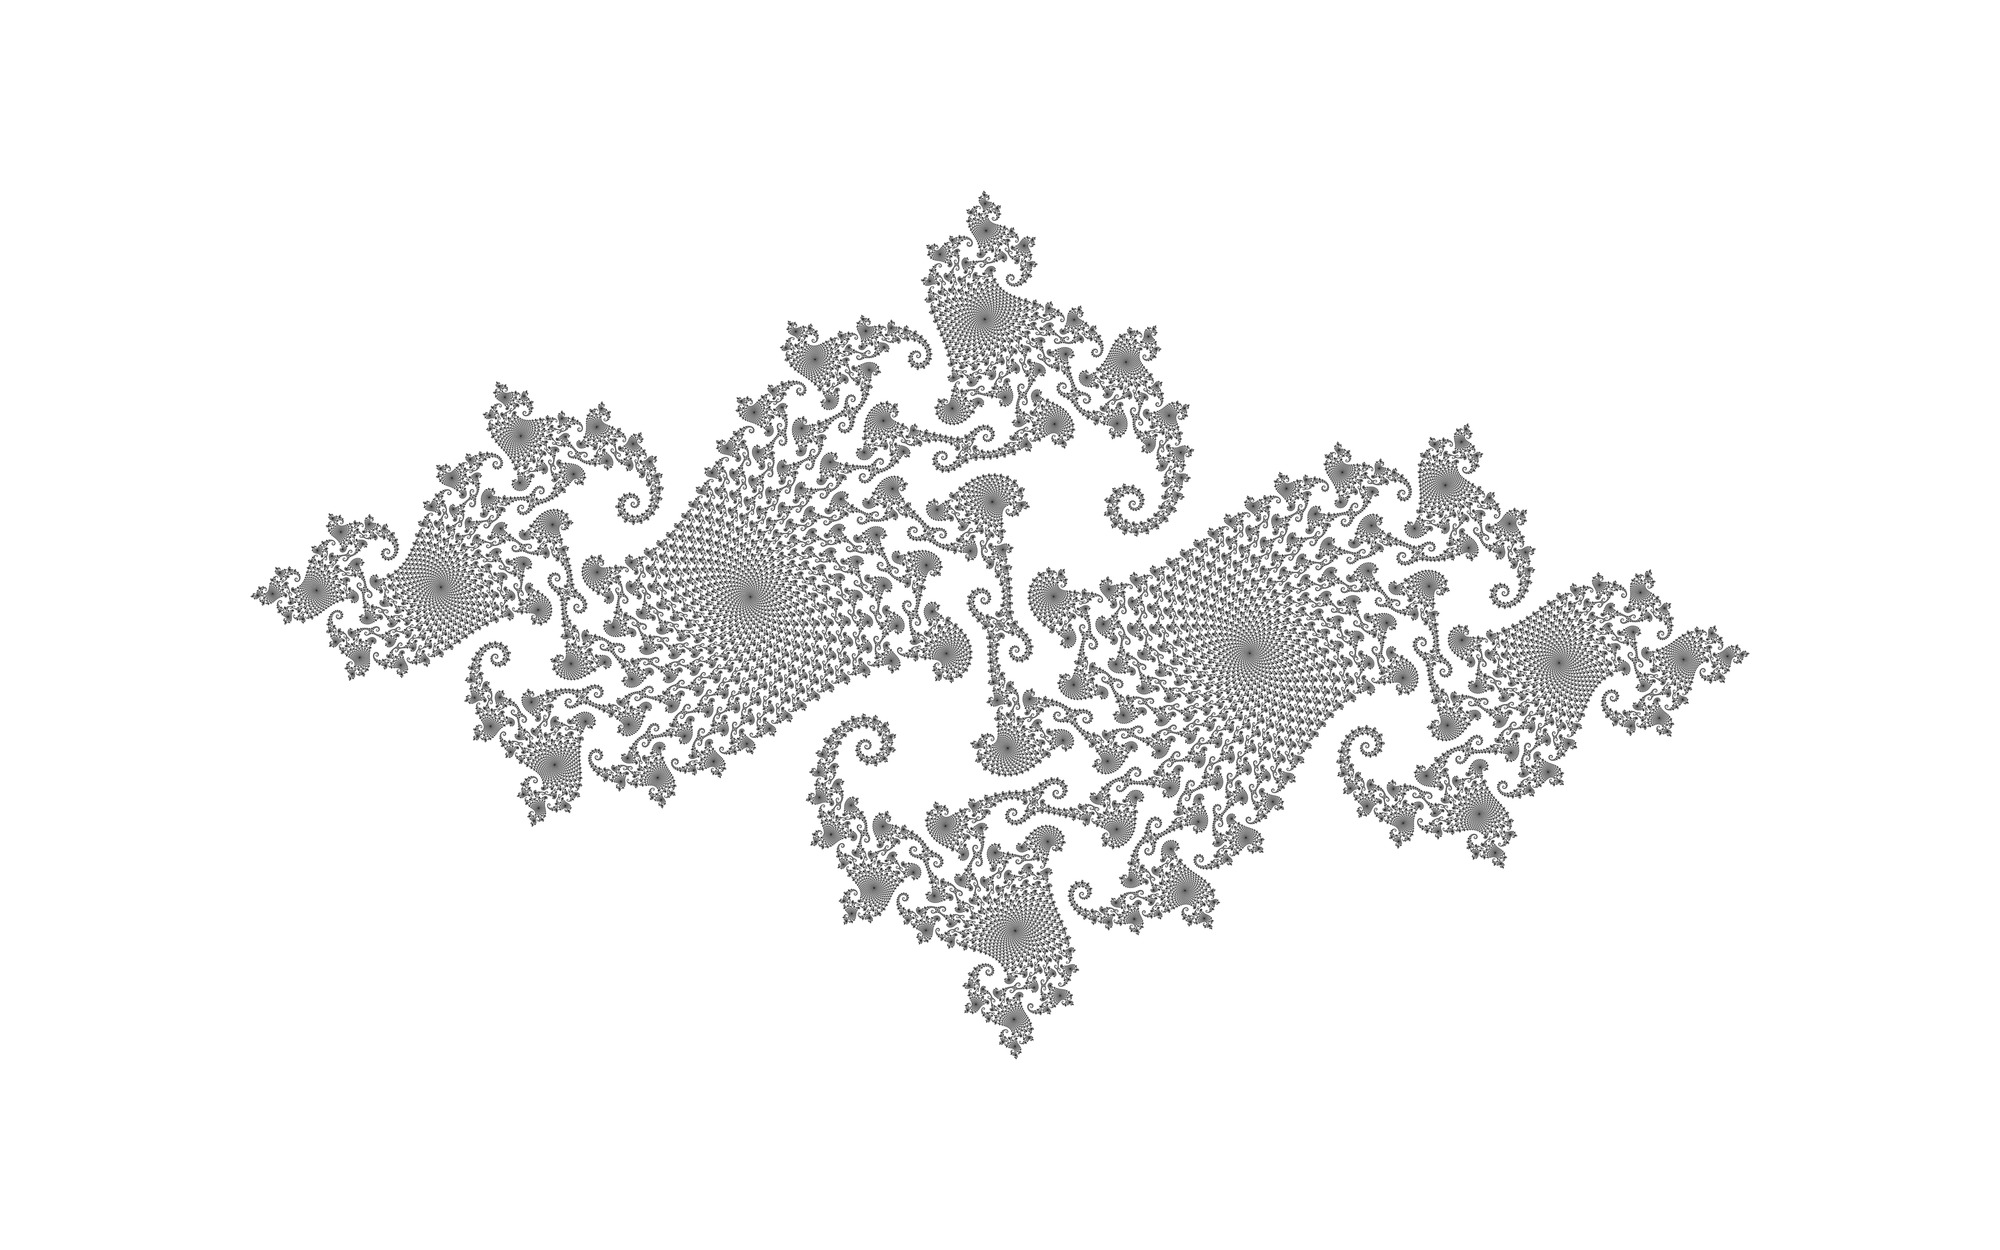
\includegraphics[width=15cm]{J4.jpg}
        \end{figure}
        
        
        Since the Julia set is non-empty and has no isolated points, the Fatou components are hyperbolic. One can now study periodic Fatou components by replacing $f$ with a suitable iterate and procuring information from dynamics on hyperbolic surfaces. Classifying dynamics on hyperbolic surfaces in itself is not interesting because of the sheer lack of chaotic behaviour; We nevertheless use the classification as a tool for studying Fatou components.    
        
        \subsection*{Theorem 2.29}{(Classification of Dynamics on Hyperbolic Surfaces)}: Let $f$ be a self map on a hyperbolic surface $S$. Exactly one of the four possibilities holds:
        \begin{enumerate}
            \item $f$ has an attracting fixed point. 
            \item For all compact sets $K$ in $S$, the iterates of $K$ eventually exit $K$.
            \item $\exists n$ such that $f^{\circ n}$ is identity.
            \item $S \cong \mathbb{D}$, $\mathbb{D}\backslash \{0\}$, or $\mathbb{A}_r := \{z|$ $1<|z|<r\}$ and $f \equiv z \rightarrow e^{2\pi i \alpha}z$ with $\alpha \notin \mathbb{Q}$.
        \end{enumerate}
        
        
        
        Three remarks are in order. First, one can lift $f$ to a map $F$ between its universal covers and apply Schwarz's lemma to get that all orbits of $F$ converge uniformly on compacts to the zero function which then can be passed on to $f$. Second, suppose $f$ is a rational map with $\deg(f)\geq2$ and has a Fatou component $U$ containing a fixed point $z$ with $|f'(z)|=1$. Then $U \cong \mathbb{D}$, and $f$ is equivalent to an irrational rotation on $\mathbb{D}$. Indeed, the attracting case is off as $|f'(z)| = 1$, the escape case is off because of compactness, the finite order case is off since the degree of $f$ is $\geq 2$, and finally as $f$ admits a fixed point in $U$, it can't be equivalent to an irrational rotation on a punctured disk or an annulus. 
        Such Fatou components are called Siegel Disks. If the Fatou component $U$ is such that $f$ on $U$ is equivalent to an irrational rotation on an annulus, we call $U$ a Herman ring. And it can easily be observed that the case of a punctured disk being a proper Fatou component shall never arise, for Julia sets don't have isolated points. Third, if $U$ were a hyperbolic forward invariant Fatou component, then the second case in the classification theorem is equivalent to the boundary convergence case described in the lemma below.
        
        \subsection*{Lemma 2.30}{(Convergence to a Boundary Fixed Point)}: Suppose $U$ is a hyperbolic domain of a compact Riemann surface and the self map $f$ on $U$ extends continuously to $\partial U$, with at most finite number of fixed points in $\partial U$. If some orbit of $f$ has no accumulation in $U$ then all orbits in $U$ converge to a boundary fixed point of $f$. Further, the convergence is uniform on compacts.
        
        
        One of the many ways to describe dynamics on a Fatou component is by reducing the function $f$ to a simpler one (in the right set of coordinates). In particular, if $U\subset S$ and $\phi: U \rightarrow \phi(U) \subseteq \mathbb{C}$ is a biholomorphism, then of all such $\phi$'s we look for the one that would have $\phi \circ f \circ \phi^{-1}$ in its simplest form. Siegel disks and Herman rings are instances of such things. Results that have the aforementioned flavour are called Linearization Theorems. One tries to turn $f$ into as linear a function as possible. This is where the philosophy we talked of runs full throttle. Usually, one studies the behaviour of $f$ in neighbourhoods $U$ of certain fixed points, and orbits of critical points show up on the boundaries of largest possible $U$. In addition to that, orbits of critical points also reveal certain topological structures of Julia sets, so do certain periodic points. Hence, fixed points and distribution of the orbits of critical points are crucial.

        Understanding dynamics of $f$ near fixed points (locally) pertains to finding a change in the coordinate system which would ease the description of orbits of $f$. A general technique in this direction is first constructing a sequence $\{\phi_k\}_k$ of biholomorphisms embedding a neighbourhood of a fixed point into $\mathbb{C}$ such that $\phi_k \circ f = g \circ \phi_{k+1}$, and then proving that $\{\phi_k\}_k$ converges uniformly to some $\phi$. We shall then have,
        $$\lim_{k \rightarrow \infty}(\phi_k \circ f) = \lim_{k \rightarrow \infty}(g \circ \phi_{k+1})$$ This establishes the fact that $\phi \circ f \circ \phi^{-1} = g$, where $g$ is a polynomial, preferably linear.

        We shall now study local behaviour of $f$ around four types of fixed points - attracting, repelling, superattracting, and parabolic. Let $\hat{f} = \phi \circ f \circ \phi^{-1}$ be a regular coordinate representation of $f$ (centered around a fixed point). Notice that $\hat{f}'(0) \notin \{0, 1\}$ $\implies$ on domains near enough to the fixed point, $f$ behaves like $\hat{f}(0)z$ (or $\lambda z$, where $\lambda $ is the multiplier). If $\lambda <1$, $f$ pulls, and if $\lambda > 1$, $f$ pushes. If $\lambda = \hat{f}'(0) = 0$, then locally $\hat{f}(z) = a_nz^n + a_{n+1}z^{n+1} + \ldots$ $\implies$ $\hat{f}$ has a zero of order $n$ at $0$. In a suitable domain, $f$ shall then behave like $(h(z)z)^n$, where $h(z)$ is non-vanishing near $0$, hence on a compact neighbourhood its modulus shall admit extreme values. Thus, one can expect $f$ to locally behave (approximately) like a polynomial. If the fixed point is parabolic (i.e $\lambda = 1$), then one should expect a totally different local behaviour. For instance, consider $(z \rightarrow z + z^3): \mathbb{C} \rightarrow \mathbb{C}$. Evidently $f$ throws off points $1, -1$, and pulls close points $i, -i$. That is, locally it seems as if points are attracted and repelled along different directions at the same time. In summary, these four types of points must be handled separately.
        
        \subsection*{Theorem 2.31}{(Koenig's Coordinates)}: Let $U$ be a sufficiently small neighbourhood around a fixed point $\hat{p}$ such that $|\lambda| \notin \{0, 1\}$, then there exists  a (unique up to multiplication by a non-zero constant) conformal embedding $\phi: U \rightarrow \mathbb{C}$ such that $(z \rightarrow \lambda z) \circ \phi = \phi \circ f$.  
        
        
        \subsection*{Theorem 2.32}{(B\"ottcher Coordinates)}: Let $U$ be a sufficiently small neighbourhood around a fixed point $\hat{p}$ such that $\lambda = 0$, then there exists  a (unique up to multiplication by a $(n-1)$st root of unity) conformal embedding $\phi: U \rightarrow \mathbb{C}$ such that $(z \rightarrow z^n) \circ \phi = \phi \circ f$, if the order of zero of the coordinate representation of $f$ at $0$ is $n$. 
        
        
        
        To do something similar for parabolic points we need to work a bit more.
        
        \subsection*{Definition 2.33}{(Attracting/Repelling Vectors)}: Let us denote the coordinate representation of $f$ by $f$ itself, and say it locally has the form $f(z) = z + az^{n+1} + O(z^{n+2})$, then $v \in \mathbb{C}$ is called an attracting vector if $nav^n = 1$ and the same is called a repelling vector if $nav^n = -1$. (Note: Since $f$ is locally invertible it can be shown that for $f^{-1}$ the roles of attracting and repelling vectors get swapped. Also, $nav^n = \pm 1$ has $2n$ equally spaced solutions, hence there are $n$ attracting and $n$ repelling (equally spaced) vectors.)
        
        
        \subsection*{Proposition 2.34}{(Attraction/Repulsion along certain Directions)}: If the orbit of $z_0$, $\{z_k\}_k$ converges to $0$, and $z_k \neq 0$, $\forall k$, then, $$z_k \sim \frac{v_j}{\sqrt[\frac{1}{n}]{k}}$$ Similarly, for orbits converging to $0$ under $f^{-1}$. 
        
       
       
       Set $v_j = e^{\frac{\pi i j}{n}}v_0$ $\implies$ $v_j$ is attracting if $j$ is odd and repelling if it is even. So, attracting and repelling vectors sandwich each other. Further, it is expected from the proposition above that some domain in $\Delta_j := \{re^{i\theta}v_j|$ $r>0, |\theta| < \frac{\pi}{n}\}$ must firstly contain an orbit $\{z_k\}_k$ and secondly must asymptotically approach $0$ along the direction $v_j$ for odd $j$. Such domains are called petals. More precisely,
       
       \subsection*{Definition 2.35}{(Petals)}: Let $N$ be a neighbourhood of the parabolic point $\hat{p}$ on which $f$ is univalent. $P \subset N$ will be called an attracting petal for $f$ at $\hat{p}$ if:
       \begin{enumerate}
           \item $f(P) \subseteq P$
           \item $\{z_k\}_k$, orbit of $z_0$ eventually enters $P$ iff $z_k \rightarrow \hat{p}$ along $v_j$. 
        \end{enumerate} 
        
           
        
        These domains (visually) look like petals around the base branch $v_j$. Such petals exist, in fact the following theorem says something far more beautiful than substantiating mere existence.
           
        \subsection*{Theorem 2.36}{(Parabolic Flower)}: $\exists$ petals $\{P_j\}_{0\leq j\leq 2n-1}$, where $P_j$ is either attracting or repelling such that $\{\hat{p}\} \cup P_0 \cup P_1 \cup \ldots \cup P_{2n-1}$ is an open neighbourhood of $\hat{p}$. Further, $P_j, P_j\cap P_{j\pm1}$ are simply connected regions (except for $n =1$).
        
        
        \begin{figure}[htp]
            \centering
            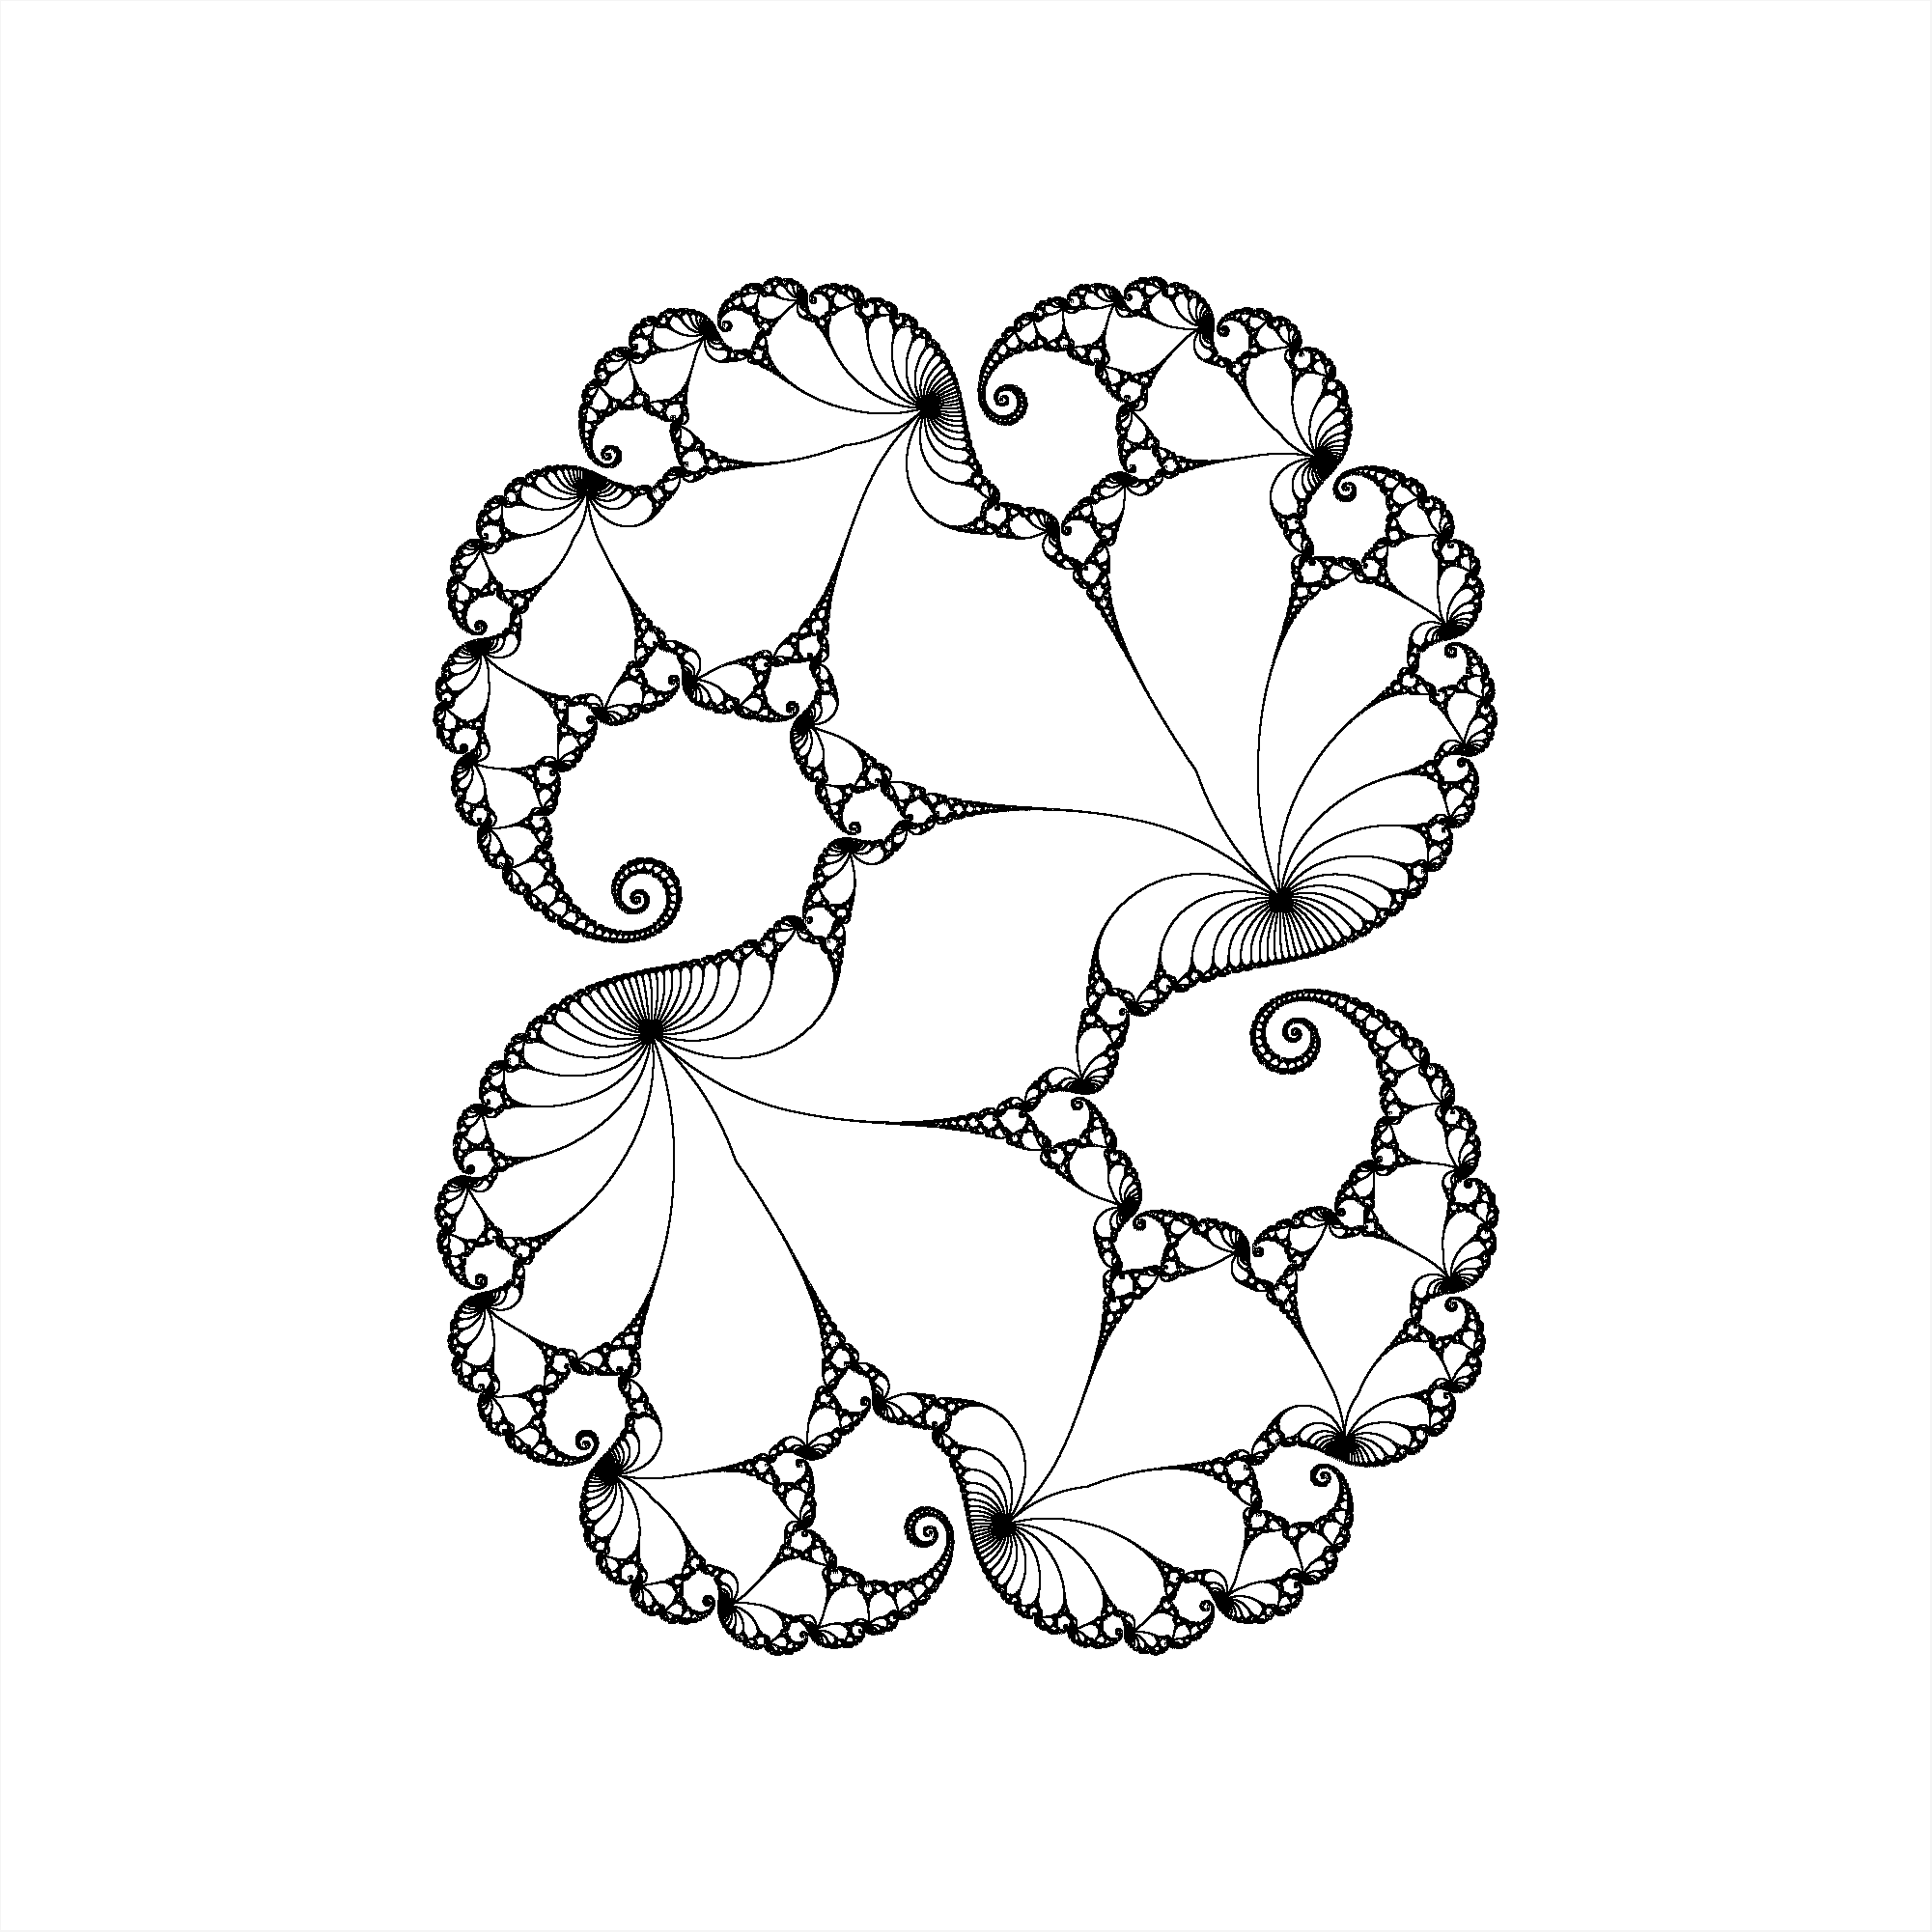
\includegraphics[width=14cm]{P.png}
        \end{figure}
        
        \subsection*{Definition 2.37}{(Parabolic Basin)}: Let $\mathcal{A}_j(\hat{p})$ for a parabolic $\hat{p}$ be the set of all $p_0$ such that $p_0 \rightarrow p_1 \rightarrow p_2 \rightarrow \ldots$ under $f$ goes to $\hat{p}$ along ${v_j}$ (the $j$th attracting vector). It is evident from the existence of petals that there exists a connected component of $\mathcal{A}_j(\hat{p})$ that is forward invariant which we shall denote by $\mathcal{A}_j^o(\hat{p})$  
        
        
        \subsection*{Theorem 2.38}{(Fatou Coordinates)}: For any petal $P$ $\exists$ (a unique up to translation) conformal embedding $\alpha: P \rightarrow \mathbb{C}$ such that $(z \rightarrow z+1) \circ \alpha = \alpha \circ f$. 
        
        
        
        We have seen the role played by fixed points so far, now let us explain the phenomenon of critical points, but for that, we have to restrict ourselves to the case of rational maps. Critical points govern the dynamics of rational maps in three significant ways:
        
        \begin{enumerate}
            \item Critical points bound the extent to which Koenigs, Fatou and B\"ottcher coordinates can be extended biholomorphically. 
            \item Number of critical points bound the number of attracting/parabolic periodic points.
            \item It determines the shape of the Julia set. 
        \end{enumerate}
            
        
        \subsection*{Theorem 2.39}
        $\exists$ maximal $r$ such that $\xi: \mathbb{D}_r \rightarrow \mathcal{A}^o$ is a holomorphic inverse of the Koenigs coordinate $\phi$, and $\xi(\partial \mathbb{D}_r)$ contains a critical point of $f$. 
        
            
        \subsection*{Theorem 2.40}
        $\exists$ a maximal petal $P_{max}$ in all immediate parabolic basins such that the Fatou coordinate $\alpha$ extends biholomorphically to $P_{max}$ and $f$ has a critical point on $\partial P_{max}$. (Note: $\hat{p}$, a parabolic fixed point being on the Julia set, shall spread its grand orbit on a dense subset bounding the maximal petal). 
        
            
        \subsection*{Corollary 2.41}
        Number of attracting and parabolic periodic points are finite.
        
            
        \subsection*{Theorem 2.42} $\exists$ maximal $r$, $0<r \leq 1$ such that the B\"ottcher coordinate $\phi$ has a holomorphic inverse $\xi$ on $\mathbb{D}_r$. If $r=1$, $\mathbb{D} \cong \mathcal{A}^o$ and $\hat{p}$ the superattracting fixed point shall be the only critical point in $\mathcal{A}^o$, else $\exists$ another in $\mathcal{A}^o$ on $\partial \xi(\mathbb{D}_r)$.
        
            
        
        For the time being let us specialize further to the case of polynomials on $\mathbb{C}$.
            
        \subsection*{Definition 2.43}{(Filled Julia Set)}: A filled Julia set is $\{z\in \mathbb{C}|$ orbit of $z$ under $f$ is bounded$\}$ (usually denoted by $K$ or $K(f)$). 
        
        
        
        Let us briefly talk about the filled Julia set of a polynomial $f(z) = a_0 + a_1z +\ldots a_dz^d$, for $d \geq 2$. Assume WLOG that $f$ is monic (else work with $cf(z/c)$). We know that one can write the filled Julia set of $f$ as $(\mathcal{A}^o(\infty))^c$. Recall the fact that the neighbourhoods of points on the Julia set are expansive upon iteration, since iterations of neighbourhoods in the interior of the filled Julia set can't escape itself, the boundary of the filled Julia set must be the Julia set of $f$. It can further be observed that all the bounded Fatou components of $f$ housed in $K$ are simply connected.
        
        \subsection*{Theorem 2.44}{(Structure of Filled Julia Set)}: $K$, $\partial K$ is connected $\iff$ All critical points have bounded orbits.
        
        
        
        As an instance of what has been put forth let us very briefly touch upon the study of dynamics of a parametrized family of self maps $\{f_{\lambda}\}_{\lambda \in \Lambda}$ on a Riemann surface $S$ for a particularly benign choice of $S$ and $f_{\lambda}$, namely, $S = \mathbb{C}$, and $f_{\lambda}(z) = z^2 + \lambda$. We know that the orbit of $0$ under $f_{\lambda}(z)$ crucially determines the topological shape of the Julia set of $f_{\lambda}(z)$. In that, if the orbit is bounded then $K(f_{\lambda}(z))$ and $J(f_{\lambda}(z))$ shall both be connected, else they shall break apart into uncountably many components. 
        
        \subsection*{Definition 2.45}{(Mandelbrot Set)}: The Mandelbrot set $\mathcal{M}$ is defined to be the set of all $\lambda$ such that the orbit $\{f_{\lambda}^{\circ n}(0)\}_n$ is bounded.
        
        
        
        Of particular interest within this set is the set of all parameters that contain a $p$-attracting cycle. The following proposition kneads such parameters together into a connected component.
        
        \subsection*{Proposition 2.46}{(Hyperbolic Components)}: Suppose there is an attracting cycle of period $m$ for $f_{\lambda}$, then $\lambda \in $ Int$(\mathcal{M})$. Further, if $\Omega$ is a component of Int$(\mathcal{M})$ containing $\lambda$, then for all $c \in \Omega$, $f_c$ contains an attracting cycle of period $m$.
        
        
        \begin{figure}[htp]
            \centering
            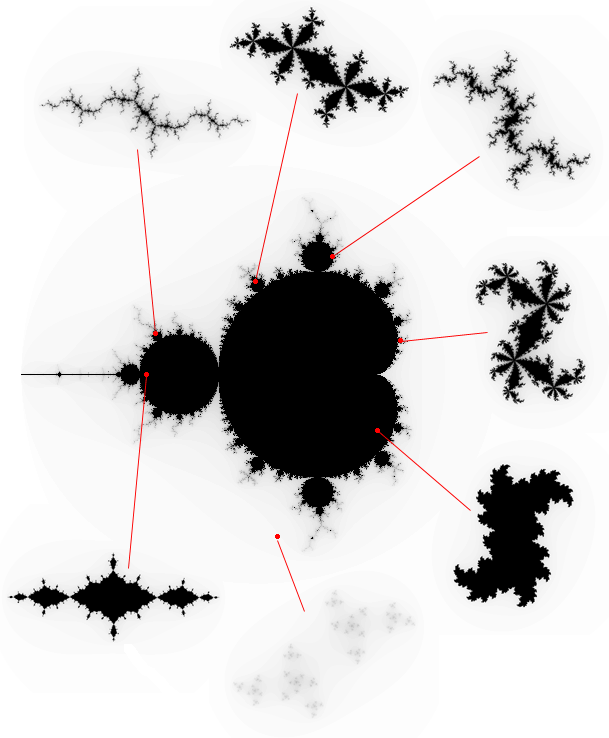
\includegraphics[width=10cm]{M4.png}
        \end{figure}
        
        
        At this juncture, let us remark that the beautiful images of Julia sets we see are constructed using density of grand orbits of certain points in it. The possibility of computer experimentation and illustration was a major factor in reviving this subject in addition to works of Fatou, Julia, Sullivan, Hubbard, and Thurston. With that context in mind, let us state this one theorem which shall be of importance to us later, and is also relevant at this stage, given the context of the philosophy we so elaborately illustrated with theorems. 
        
        \subsection*{Theorem 2.47} For a rational map $f$ with degree at least $2$, the closure of the set of repelling periodic points equals the Julia set of $f$.
        
        
        
        Having developed the theory so far, let us state its first classification theorem. The image of a Fatou component $U$ under $f$ is also a Fatou component. Indeed, if $f(U) \subset U'$, where $U'$ is some other Fatou component then given $x \in f(U)$, $y \in f(U)^c\cap U'$, $\exists$ a path in $U'$ joining $x$ and $y$. That path must hit $\partial f(U)$ on its way, contradicting the fact that the Fatou set and the Julia set are disjoint. Having said this, we note that a Fatou component $U$ can do one of the following four things:
        \begin{enumerate}
            \item $f(U) = U$ (invariant Fatou component).
            \item $f^{\circ n}(U) = U$ (periodic Fatou component).
            \item $f^{\circ k}(f^{\circ n}(U)) = f^{\circ n}(U)$ (preperiodic Fatou component).
            \item Elements in $\{f^{\circ n}(U)\}_n$ are pairwise disjoint. (wandering Fatou component).
        \end{enumerate} 
        
        \subsection*{Theorem 2.48}{(Classification of Non-Wandering Fatou Components)}: Let $U$ be a non-wandering Fatou component then it is either a branched covering or a biholomorphic copy of some periodic Fatou component, which necessarily belongs to one of the following categories:
        \begin{enumerate}
            \item $U$ is an immediate basin of attraction of some attracting cycle.
            \item $U$ is an immediate parabolic basin of attraction of some parabolic cycle.
            \item Under a suitable iterate of $f$, $U$ is a Siegel disk.
            \item Under a suitable iterate of $f$, $U$ is a Herman ring.
        \end{enumerate}
% BLOG-CONTENT-END
\bibliographystyle{amsalpha}
\bibliography{tools/profiles/surgeries/MSc_Dissertation}
\end{document}
